\documentclass[11pt, a4paper]{article}

\usepackage[utf8]{inputenc}
\usepackage{authblk}
\usepackage{titlesec}

% Maths tools
\usepackage{amsmath}
\usepackage{amssymb}

% Margin
\usepackage[margin=2.9cm]{geometry}

% Line numbers
\usepackage{lineno}

%Scientific notation
\usepackage{siunitx}

% Spacing
\usepackage{setspace}
\doublespacing

% Enumeration
\usepackage{enumerate}

% indentation
\setlength\parindent{10pt}
\setlength{\parskip}{5pt}

% Figures
\usepackage{graphicx}
\usepackage{caption}
\usepackage{subcaption}
\usepackage{epstopdf}
\renewcommand{\thefigure}{\textbf{\arabic{figure}}}
\renewcommand{\figurename}{\textbf{Supplementary Figure}}

%table
\usepackage{multirow}
\usepackage{hhline}
\usepackage[table]{xcolor}
\renewcommand{\thetable}{\textbf{\arabic{table}}}
\renewcommand{\tablename}{\textbf{Supplementary Table}}

%footnotes
\usepackage{footmisc}
\renewcommand{\thefootnote}{\fnsymbol{footnote}}

% References
\usepackage[sort&compress, numbers,super]{natbib}
\bibliographystyle{unsrtnat}
\PassOptionsToPackage{hyphens}{url}\usepackage[colorlinks=true,linkcolor=magenta, citecolor=magenta]{hyperref}
\renewcommand\refname{Supplementary References}

%subsubsection format
\titleformat*{\subsubsection}{\large\it}

%highlighting text
\usepackage{color, xcolor,soul}
\definecolor{blau}{RGB}{236,226,240}
\soulregister\cite7
\soulregister\citet7
\soulregister\citealt7
\soulregister\citenum7
\soulregister\citep7
\soulregister\ref7
\DeclareRobustCommand{\hlc}[1]{{\sethlcolor{blau}\hl{#1}}}

\usepackage{titlesec}% http://ctan.org/pkg/titlesec
\titleformat{\section}%
  [hang]% <shape>
  {\normalfont\bfseries\Large}% <format>
  {}% <label>
  {0pt}% <sep>
  {}% <before code>
  
\renewcommand{\thesection}{}% Remove section references...
\renewcommand{\thesubsection}{}%... from subsections
  \renewcommand{\thesubsubsection}{Supplementary Method \arabic{subsubsection}:}%... from subsections


  
%Title paper
\title{\vspace{-1cm} \normalsize Supplementary Information\\\vspace{0.2cm}
\LARGE Basic aspects of species' distributions}

\author{\textit{Bramon Mora and Alexander}}

\date{}

\begin{document}
\maketitle
\thispagestyle{empty}

\clearpage

% Full description of Binomial model with multiple environmental covariates
% Full description of Categorical model with multiple environmental covariates
% Full description of Categorical model with heavy-tails---generalized error distribution
% Full description of Categorical model with heavy-tails---Student's t-distribution
% Full description of Categorical model with skewed---skewed normal distribution
% Using a MMSBM to calculate species similarity
% Edge problem in stan and need to define minimum probability.

\section*{Supplementary Methods}
\subsubsection*{Distance matrices from incomplete categorical and ordinal data}
The prior information that we have regarding species' distributions is represented by the set of ordinal and categorical traits found in the floristic database. More specifically, both the ecological indicator values and range of variation are ordinal traits specified for all species, whereas plants' physiological data are characterized by categorical data containing multiple missing entries. These data could be directly used as covariates in any given distribution model; however, we want this information to be accounted for as a prior for the parameters of our Bayesian model. To do so, we need to compile the traits in the floristic database into variance-covariance matrices characterizing the \textit{a priori} similarity between species.

The missing component in the description of model (\ref{eq:baseline}) is the distance matrices $D^{\chi}$ used to define the covariance matrices $\Sigma^{\alpha}$, $\Sigma^{\beta_{k}}$ and $\Sigma^{\lambda_{k}}$. In this model, such distance matrices characterize differences between plant species. In the floristic data, however, the prior information that we have for these differences is represented by a set of ordinal and categorical traits. More specifically, both the ecological indicator values and range of variation---which define the prior information that we have for $\beta_i^k$, and $\lambda_i^k$, respectively---are ordinal traits specified for all species. In contrast, the plants' physiological data---shaping the prior for the parameters $\alpha_i$---are characterized by categorical data containing multiple missing entries. Therefore, we need to carefully compile this data into distance matrices in order to be able to feed this prior information into the model. 

More generally, we want to understand the way $N$ species are characterized by $M$ categorical traits. One way to frame this problem is by using a network representation. Following the ideas presented by \citet{godoy-loriteAccurateScalableSocial2016}, we assume that species can be connected to each of these traits by an interaction $\left(i, j\right)$ that can be of any type $r\in R$. Notice that this provides as with multiple ways to account for the information---and lack thereof---contained in the different categorical and ordinal traits $M$. That is, the $R$ types of interactions can represent the lack of information for a particular link $\left(i, j\right)$, the absence or presence of such interaction, and any type of association between $i$ and $j$. 

Given a set of interactions $R^{*}$ between $N$ and $M$, we use a Mixed Membership Stochastic Block Model (MMSBM) to characterize these. In particular, we consider that plants and traits can be classified into $K$ and $L$ groups, respectively. For every species $i$, we assume that there is a probability $\theta_{i\alpha}$ for it to belong to any of the $K$ species groups. Likewise, we also assume that any trait $j$ has a probability $\phi_{j\beta}$ of belonging to any of the $L$ trait groups. Finally, we define $p_{\alpha\beta}\left(r\right)$ as the probability of a species from group $\alpha$ interacting with a trait from group $\beta$ by an association type $r$. Putting these together, the probability of an interaction $\left(i, j\right)$ of type $r$ can be calculated as:
\begin{equation}
Pr[r_{ij}=r] = \sum_{\alpha \beta} \theta_{i\alpha} \phi_{j\beta} p_{\alpha\beta}\left(r\right)
\end{equation}
Following this definition, we want to find the group memberships that maximize the likelihood $P\left(R^{*}|\theta, \phi, p\right)$. Doing so is difficult optimization problem; however, it has been shown that one can estimate the different $\theta_{i\alpha}$, $\phi_{j\beta}$, and $p_{\alpha\beta}\left(r\right)$ parameters by maximizing the likelihood using an expectation-maximization algorithm \citep{godoy-loriteAccurateScalableSocial2016, tarres-deulofeuTensorialBipartiteBlock2019}. In simple terms, one can iteratively find multiple local minima for the likelihood, and average over the estimated the parameter values \citep{godoy-loriteAccurateScalableSocial2016}\footnote[2]{
While this averaging is trivial for the estimated probabilities $Pr[r_{ij}=r]$, it is non-trivial if one wants to find averages for the group memberships. The reason for this is related to the stochastic nature of the expectation-maximization algorithm. This algorithm initially assigns random group memberships to both species and traits. While this random labelling is irrelevant when studying the probabilities $Pr[r_{ij}=r]$, it is instead crucial for averaging $\theta_{i\alpha}$, $\phi_{j\beta}$, and $p_{\alpha\beta}\left(r\right)$. Therefore, before averaging the group membership estimates, one needs to find the bijective relationship for the labellings of different iterations of the optimization algorithm. In a nutshell, for every iteration, I do this by using a simulated annealing algorithm on the estimated $p_{\alpha\beta}\left(r\right)$, matching the corresponding labelling to a reference iteration.}. 

The average estimates for the group memberships provide us with a different scale to classify species based on the traits these have. In short, for any species $i$, we can estimate a $K$-dimensional vector $\vec{\theta}_{i}$ that describes the extend to which $i$ belong to each group membership---i.e. the extend to which a species is of one type or another. This classification is useful because it can be used to compare species, defining a way to measure the distance between species based on an arbitrary---and potentially incomplete---set of categorical or ordinal traits $M$. The simplest case is to define the distance as $D_{ij} = |\vec{\theta}_{i}-\vec{\theta}_{j}|$. Alternatively, one could also define $K$ distance matrices based on the different group memberships $D^{\alpha}_{ij} = |\theta_{i\alpha}-\theta_{j\alpha}|$.

\section*{Supplementary Notes}
\section*{Supplementary Figures}

\begin{figure}[ht]
  \centering
    \vspace{0.5cm}
    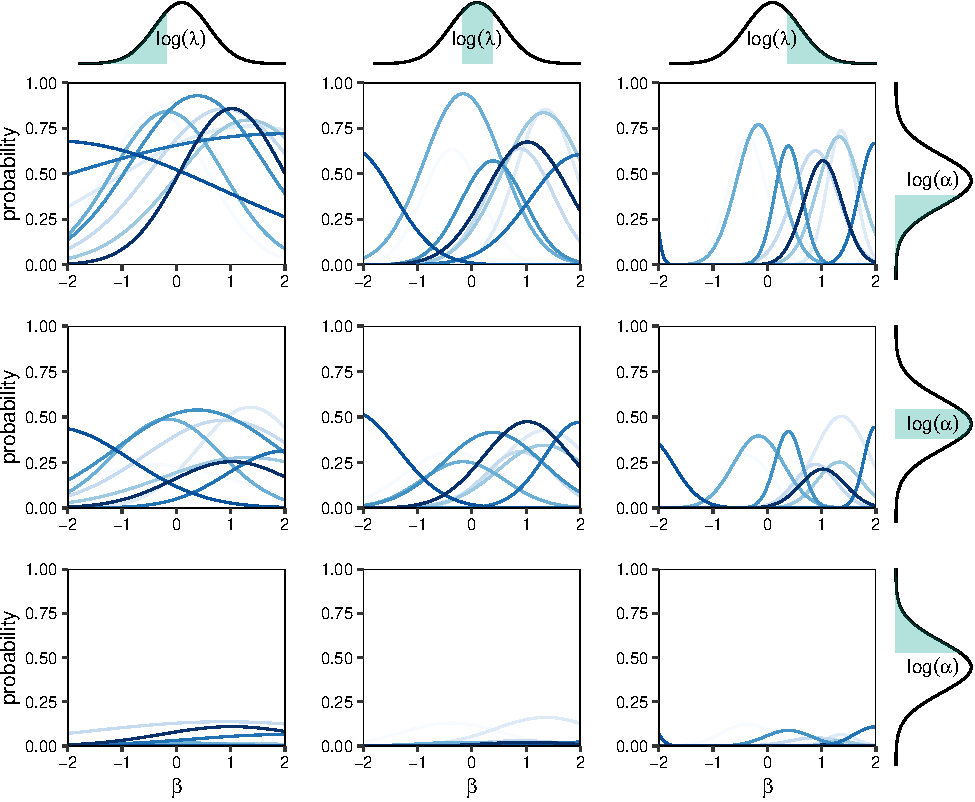
\includegraphics[width=1\textwidth]{figures/prior}
    	  \vspace{0.3cm}
	   \caption{Study of the priors for the baseline model presented in the main text.}
      \label{sfig:sensitivity}
\end{figure}

\clearpage

\begin{figure}[h]
  \centering
    \vspace{0.5cm}
    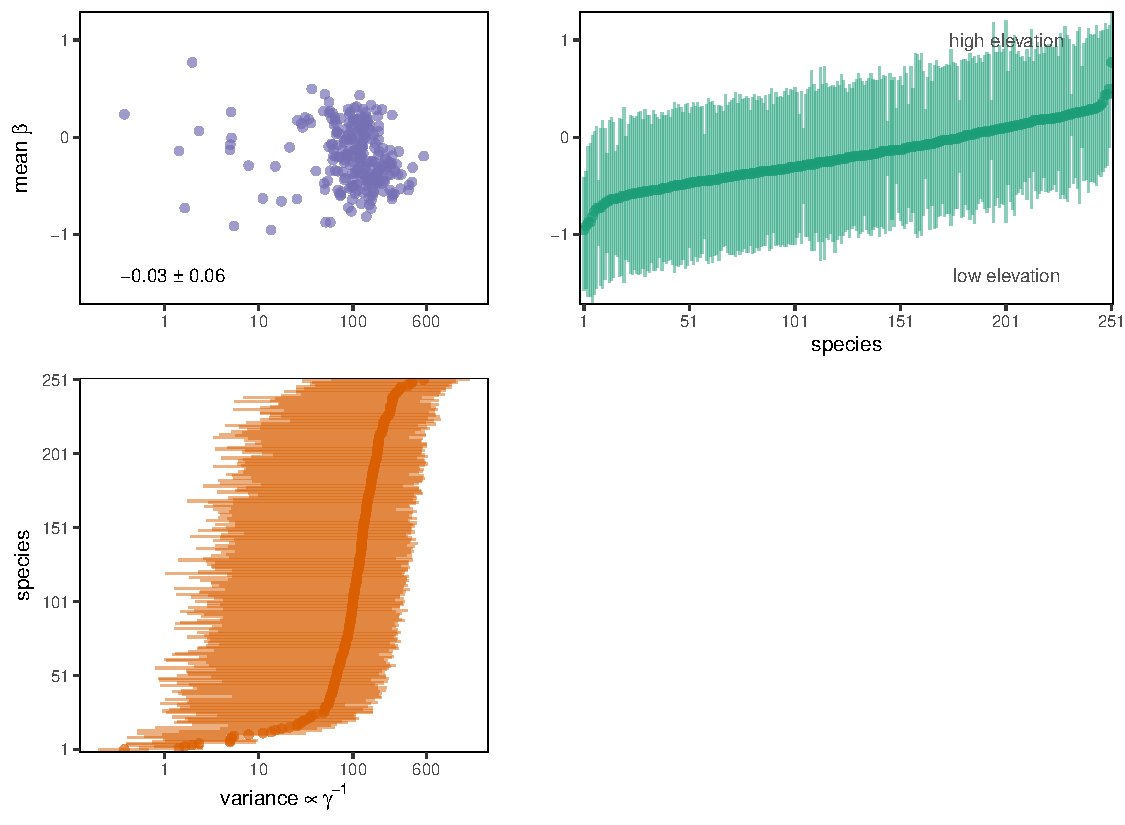
\includegraphics[width=1\textwidth]{figures/figure1-secondaxis}
    	  \vspace{0.3cm}
	   \caption{Relationship between mean and variance of species' distributions. These are the results for the second axis of variation for the climatic data.}
      \label{sfig:sensitivity}
\end{figure}

\clearpage

\bibliography{references_ab}

\end{document}
